% !TEX TS-program = pdflatex
% !TEX encoding = UTF-8 Unicode

\documentclass[11pt]{article} % use larger type; default would be 10pt

\usepackage[utf8]{inputenc} % set input encoding (not needed with XeLaTeX)
\usepackage[italian]{babel}

\usepackage{listings}
\usepackage{color}
\definecolor{bluekeywords}{rgb}{0,0,1}
\definecolor{greencomments}{rgb}{0,0.5,0}
\definecolor{redstrings}{rgb}{0.64,0.08,0.08}
\definecolor{xmlcomments}{rgb}{0.5,0.5,0.5}
\definecolor{types}{rgb}{0.17,0.57,0.68}
\lstset{language=[Sharp]C,
captionpos=b,
%numbers=left, %Nummerierung
%numberstyle=\tiny, % kleine Zeilennummern
frame=lines, % Oberhalb und unterhalb des Listings ist eine Linie
showspaces=false,
showtabs=false,
breaklines=true,
showstringspaces=false,
breakatwhitespace=true,
escapeinside={(*@}{@*)},
commentstyle=\color{greencomments},
morekeywords={partial, var, value, get, set},
keywordstyle=\color{bluekeywords},
stringstyle=\color{redstrings},
basicstyle=\ttfamily\small,
}

\usepackage{tikz}
\usetikzlibrary{shapes.geometric, arrows}
\tikzstyle{startstop} = [rectangle, rounded corners, minimum width=3cm, minimum height=0.8cm,text centered, draw=black, fill=red!30]
\tikzstyle{io} = [trapezium, trapezium left angle=70, trapezium right angle=110, minimum width=3cm, minimum height=0.8cm, text centered, draw=black, fill=blue!30]
\tikzstyle{process} = [rectangle, minimum width=3cm, minimum height=0.8cm, text centered, draw=black, fill=orange!30]
\tikzstyle{decision} = [diamond, minimum width=3cm, minimum height=0.8cm, text centered, draw=black, fill=green!30]
\tikzstyle{arrow} = [thick,->,>=stealth]
\usepackage{pgfplots}
\pgfplotsset{compat=1.12}

%%% PAGE DIMENSIONS
\usepackage{geometry}
\geometry{a4paper}
\usepackage{graphicx}
\usepackage{fullpage}

%%% PACKAGES
\usepackage{booktabs} % for much better looking tables
\usepackage{array} % for better arrays (eg matrices) in maths
\usepackage{paralist} % very flexible & customisable lists (eg. enumerate/itemize, etc.)
\usepackage{verbatim} % adds environment for commenting out blocks of text & for better verbatim
\usepackage{subfig} % make it possible to include more than one captioned figure/table in a single float
\usepackage{amsmath}
\usepackage[capposition=top]{floatrow}

%%% HEADERS & FOOTERS
\usepackage{fancyhdr} % This should be set AFTER setting up the page geometry
\pagestyle{fancy} % options: empty , plain , fancy
\renewcommand{\headrulewidth}{0pt} % customise the layout...
\lhead{}\chead{}\rhead{}
\lfoot{}\cfoot{\thepage}\rfoot{}

%%% ToC (table of contents) APPEARANCE
\usepackage[nottoc,notlof,notlot]{tocbibind} % Put the bibliography in the ToC
\usepackage[titles,subfigure]{tocloft} % Alter the style of the Table of Contents
\renewcommand{\cftsecfont}{\rmfamily\mdseries\upshape}
\renewcommand{\cftsecpagefont}{\rmfamily\mdseries\upshape} % No bold!

%%% END Article customizations

%%% The "real" document content comes below...

\title{Attrito Viscoso: una simulazione informatica}
\author{Jonatan Della Regina, Giulia Scocco, Giulio Zausa}

\begin{document}
\maketitle
\tableofcontents

\section{Introduzione}
Your text goes here.

\subsection{Descrizione Fisica}
More text.

\section{Simulazione}
Abbiamo simulato, usando il modello fisico sopra descritto, il comportamento di un oggetto che cade in un fluido viscoso. Per fare ciò abbiamo sviluppato un software che, date le costanti fisiche $g$, $\mu$ e $m$, calcoli $n$ valori di Velocità, Tempo e Accelerazione per poter disegnare un grafico Velocità/Tempo sullo schermo, e trovare approssimativamente il valore della velocità terminale.\par

\begin{center}
\begin{tikzpicture}[node distance=2cm]
\node (start) [startstop] {Inizio};
\node (input) [io, below of=start] {$I: g, \mu, m$};
\node (assign) [process, below of=input] {$t[0] \leftarrow 0, v[0] \leftarrow 0, a[0] \leftarrow g, i \leftarrow 0$};
\node (cycle) [decision, below of=assign] {$i < n$};
\node (tim) [process, right of=cycle, xshift=3cm] {$t[i] \leftarrow t + dt$};
\node (vel) [process, below of=tim] {$v[i] \leftarrow v + a * dt$};
\node (acc) [process, below  of=vel] {$a[i] \leftarrow g - \mu/m * v$};
\node (i) [process, below  of=acc] {$i \leftarrow i + 1$};
\node (output) [io, below of=cycle, yshift=-5.5cm] {$O: valori, grafico$};
\node (stop) [startstop, below of=output] {Fine};
\draw [arrow] (start) -- (input);
\draw [arrow] (input) -- (assign);
\draw [arrow] (assign) -- (cycle);
\draw [arrow] (output) -- (stop);
\draw [arrow] (tim) -- (vel);
\draw [arrow] (vel) -- (acc);
\draw [arrow] (acc) -- (i);
\draw [arrow] ([xshift=-1.5cm]i.center) -- (cycle);
\draw [arrow] (cycle) -- node[anchor=east] {no} (output);
\draw [arrow] (cycle) -- node[anchor=south] {sì} (tim);
\end{tikzpicture}
\end{center}

Questo algoritmo riempie una tabella con $n$ valori di tempo, velocità e accelerazione. Disegna inoltre il grafico Velocità/Tempo. Possiamo notare la costante $dt$, che rappresenta la differenza di tempo tra ogni campione e, in un certo senso, la risoluzione del grafico. Ci siamo accorti però che con certi valori di $dt$ il grafico cambiava radicalmente, rappresentando valori errati rispetto al modello fisico. Questo è dato dalle formule(1) usate per calcolare velocità e accelerazione:
\begin{equation}\begin{split}a_{1}=g-\frac{\mu}{m}*v_{0}\\
\text{con }v_{0}=g*dt \rightarrow a_{1}=g-\frac{\mu}{m}*g*dt\end{split}\end{equation}
L'accelerazione del corpo deve diminuire tendendo a 0 per rispettare le leggi fisiche, ma ciò non avviene se $dt > \tau$. Ricaviamo $\tau$ ponendo l'accellerazione nel secondo campione pari a zero:
\begin{equation}\begin{split} a_{1}=g-\frac{\mu}{m}*g*\tau=0\\ \tau = \frac{m}{\mu}\end{split}\end{equation}

Variando il valore di $dt$ rispetto a $\tau$, il grafico cambia forma in questo modo:\par
\begin{table}[h]
\begin{tabular}{lll}
$dt < \tau$ 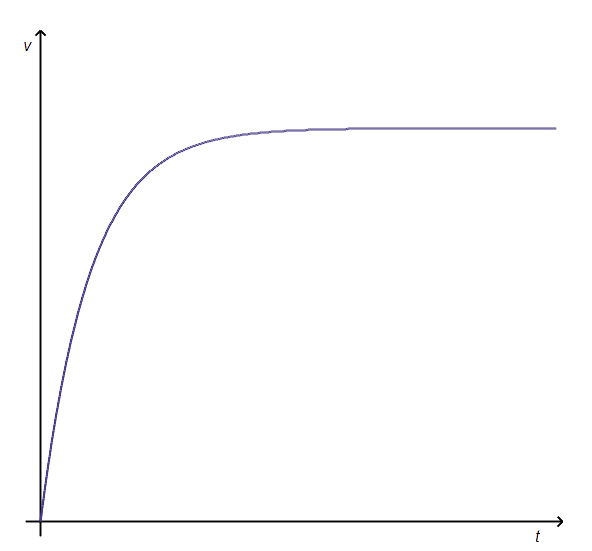
\includegraphics[scale=0.4]{1.png} & $dt = \tau$ 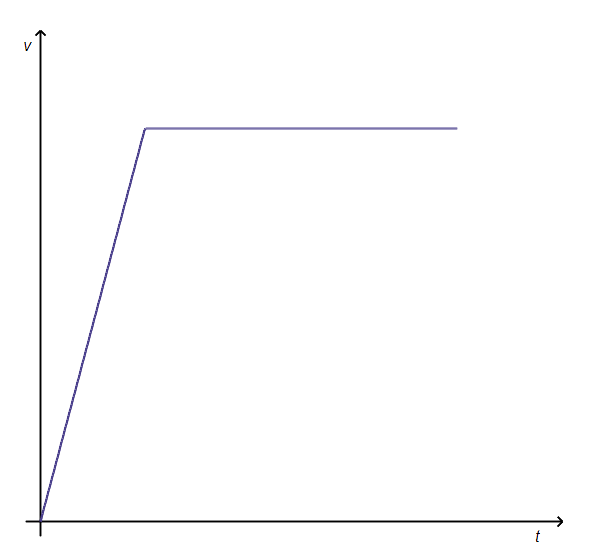
\includegraphics[scale=0.4]{2.png} \\
$dt > \tau$ 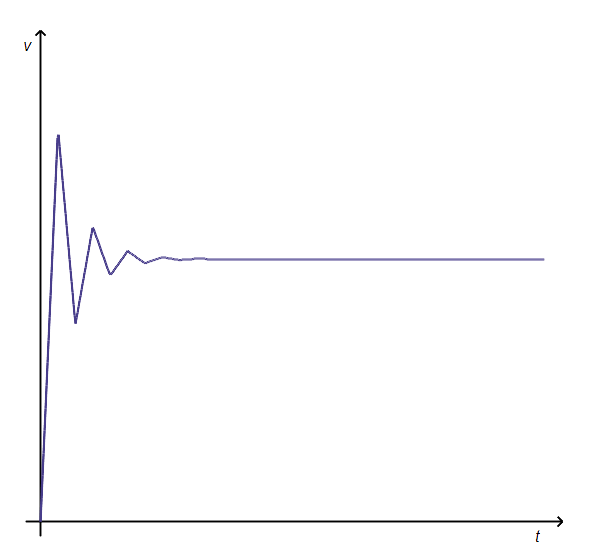
\includegraphics[scale=0.4]{3.png} & $dt = 2\tau$ 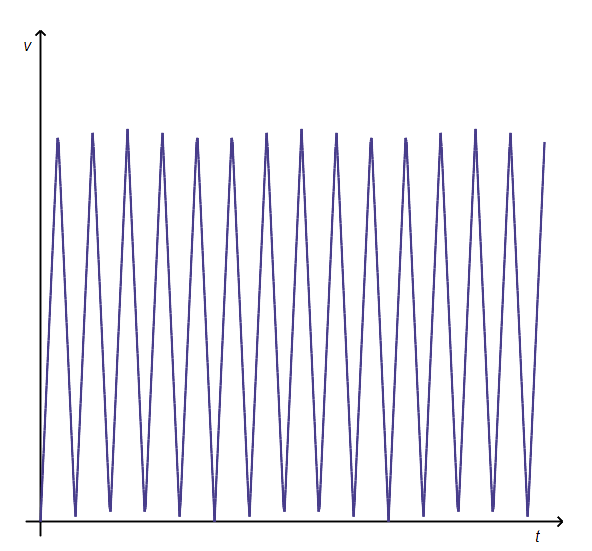
\includegraphics[scale=0.4]{4.png} \\
$dt > 2\tau$ 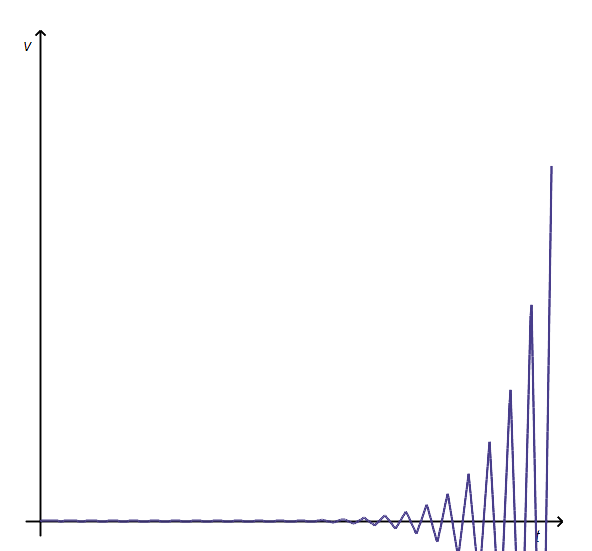
\includegraphics[scale=0.4]{5.png}
\end{tabular}
\end{table}
Per fornire all'utente un grafico che rappresenti in maniera accurata il fenomeno fisico abbiamo strutturato il programma in modo che visualizzi un avviso nel caso $dt > \tau$, e visualizzi una previsione del grafico in base ai valori di $m$ e $\mu$

\newpage
\subsection{Calcolo di $\tau$}
Per calcolare il valore approssimato di $\tau$ abbiamo usato un algoritmo che si basa su approssimazioni successive, riducendo o aumentando il valore di $dt$ fino a quando $a$ non sia pari a $0$.
\begin{center}
\begin{tikzpicture}[node distance=2cm]
\node (start) [startstop] {Inizio};
\node (input) [io, below of=start] {$I: dt, g, \mu, m$};
\node (assign) [process, below of=input] {$tdt \leftarrow dt, i \leftarrow 1$};
\node (acc) [process, below of=assign] {$a \leftarrow g - \mu / m * g * tdt$};
\node (nz) [decision, below of=acc] {$tdt = 0$};
\node (nz2) [process, right of=nz, xshift=3cm] {$tdt \leftarrow 0.1$};
\node (mi) [decision, below of=nz] {$a<0$};
\node (mi2) [process, right of=mi, xshift=3cm] {$tdt \leftarrow tdt - tdt / i$};
\node (ma) [decision, below of=mi] {$a>0$};
\node (ma2) [process, right of=ma, xshift=3cm] {$tdt \leftarrow tdt + tdt / i$};
\node (eq) [decision, below of=ma] {$a=0$};
\node (i2) [process, right of=mi2, xshift=2cm] {$i \leftarrow i + 1$};
\node (output) [io, below of=eq] {$O: \tau (tdt)$};
\node (stop) [startstop, below of=output] {Fine};
\draw [arrow] (start) -- (input);
\draw [arrow] (input) -- (assign);
\draw [arrow] (assign) -- (acc);
\draw [arrow] (output) -- (stop);
\draw [arrow] (acc) -- (nz);
\draw [arrow] (nz2) -| (i2);
\draw [arrow] (mi2) -- (i2);
\draw [arrow] (ma2) -| (i2);
\draw [arrow] (i2) |- (acc);
\draw [arrow] (nz) -- node[anchor=south] {sì} (nz2);
\draw [arrow] (ma) -- node[anchor=south] {sì} (ma2);
\draw [arrow] (mi) -- node[anchor=south] {sì} (mi2);
\draw [arrow] (nz) -- node[anchor=east] {no} (mi);
\draw [arrow] (mi) -- node[anchor=east] {no} (ma);
\draw [arrow] (ma) -- node[anchor=east] {no} (eq);
\draw [arrow] (eq) -| node[anchor=north] {no} (i2);
\draw [arrow] (eq) -- node[anchor=east] {sì} (output);
\end{tikzpicture}
\end{center}
\newpage
Che si traduce nella seguente funzione C\#:
\begin{lstlisting}
private float TauFromData(float dt, float g, float mua, float m)
{
    float tdt = dt; // dt temporaneo
    for (float i = 1f; i < 1000000; i++) // Limita un numero massimo di cicli
    {
        float a = g - mua / m * g * tdt; // Calcola accelerazione
        tdt = tdt == 0 ? 0.1f : tdt; // Evita che tdt sia 0
        if (a < 0)
            tdt -= tdt / i;
        else if (a > 0)
            tdt += tdt / i;
        else break;
        i++;
    }
    return tdt;
}
\end{lstlisting}

\subsection{Calcolo di $V_t$}
Per calcolare il valore approssimato di $V_t$(Velocità terminale) abbiamo usato un algoritmo che si basa su approssimazioni successive:
\begin{center}
\begin{tikzpicture}[node distance=2cm]
\node (start) [startstop] {Inizio};
\node (input) [io, below of=start] {$I: v[], \epsilon, n$};
\node (assign) [process, below of=input] {$i \leftarrow 1$};
\node (cycle) [decision, below of=assign] {$i < n$};
\node (check) [decision, right of=cycle, xshift=3cm] {$v_i - v_{i - 1}$};
\node (output) [io, below of=check] {$O: v_i$};
\node (output2) [io, below of=cycle] {$O: \infty$};
\node (stop) [startstop, below of=output] {Fine};
\draw [arrow] (start) -- (input);
\draw [arrow] (input) -- (assign);
\draw [arrow] (assign) -- (cycle);
\draw [arrow] (output) -- (stop);
\draw [arrow] (output2) |- (stop);
\draw [arrow] (cycle) -- node[anchor=east] {no} (output2);
\draw [arrow] (cycle) -- node[anchor=south] {sì} (check);
\draw [arrow] ([yshift=1.1cm]check.center) -- node[anchor=south] {no} ([yshift=1.1cm]cycle.center);
\draw [arrow] (check) -- node[anchor=east] {sì} (output);
\end{tikzpicture}
\end{center}
\newpage
Che si traduce nella seguente funzione C\#:
\begin{lstlisting}
private float VtFromData(float[] v)
{
    for (int i = 1; i < v.Length; i++)
    {
        if (v[i] - v[i - 1] < epsilon) // Se differenza < epsilon
        {
            return v[i];
        }
    }
    return float.PositiveInfinity;
}
\end{lstlisting}

\section{Realizzazione Grafica}
Per sviluppare il software abbiamo scelto il linguaggio C\# e le librerie di programmazione .NET Framework. Abbiamo fatto questa scelta a discapito del C++ per avere delle funzioni grafiche più potenti e più semplici.\par
\begin{center}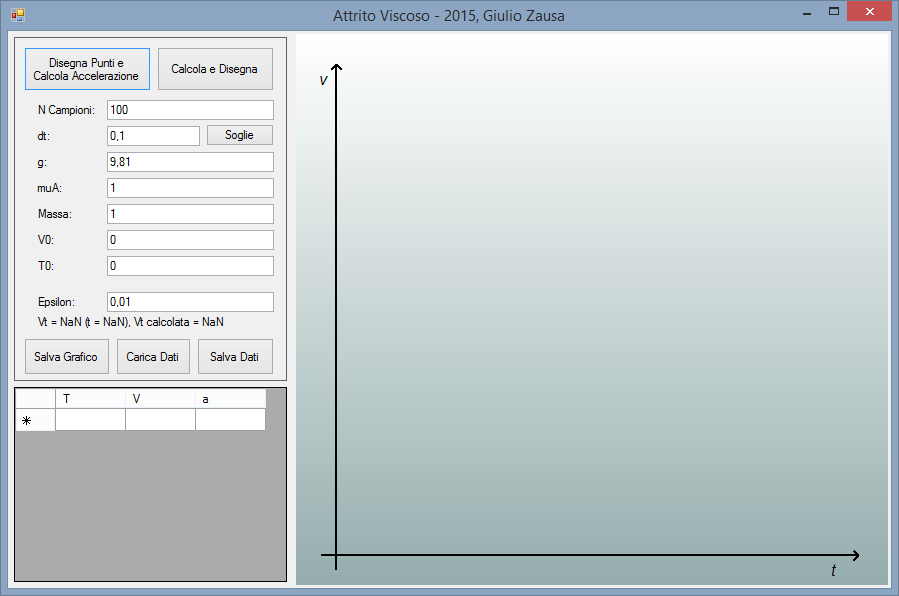
\includegraphics[scale=0.6]{screen.png}\par La form principale del programma.\end{center}
Si possono distinguere tre pannelli principali del programma:
\begin{itemize}
  \item Tabella dei Valori
  \item Grafico
  \item Pannello comandi e inserimento dati
\end{itemize}
\newpage
\section{Appendice: Codice sorgente}
\subsection{Program.cs}
\begin{lstlisting}
using System;
using System.Windows.Forms;

namespace ProGruppoInfo
{
    class Program
    {
        [STAThread]
        static void Main(string[] args)
        {
            Application.EnableVisualStyles();
            Application.SetCompatibleTextRenderingDefault(false);
            Application.Run(new MainForm());
        }
    }
}
\end{lstlisting}
\subsection{MainForm.cs}
\begin{lstlisting}
using System;
using System.Collections.Generic;
using System.ComponentModel;
using System.Drawing;
using System.Drawing.Drawing2D;
using System.Windows.Forms;

namespace ProGruppoInfo
{
    public partial class MainForm : Form
    {
        int n = 0;
        public static float dt, g, mua, m, v0, t0, epsilon, vt, tf;
        Bitmap bitmap, buffer, soglieb;
        Graphics gr;
        float maxY, maxX;
        Point origin;
        Point[] points;
        PointF[] originalPoints;
        SoglieView soglieForm;

        #region Inizializzazione
        public MainForm() // Costruttore
        {
            InitializeComponent();
            soglieForm = new SoglieView();
        }

        private void panel2_Paint(object sender, PaintEventArgs e) // Prepara buffer e disegna sfondo iniziale
        {
            bitmap = new Bitmap(panel2.Width, panel2.Height);
            buffer = new Bitmap(panel2.Width, panel2.Height);
            gr = Graphics.FromImage(bitmap);
            DrawAxes();
            panel2.CreateGraphics().DrawImage(bitmap, 0, 0);
        }

        private void MainForm_ResizeEnd(object sender, EventArgs e) // Aggiorna dimensione buffer se form ingrandita
        {
            bitmap = new Bitmap(panel2.Width, panel2.Height);
            gr = Graphics.FromImage(bitmap);
            DrawAxes();
            panel2.CreateGraphics().DrawImage(bitmap, 0, 0);
        } 
        #endregion

        #region Disegno Grafici
        // Disegna i dati
        private void DrawData()
        {
            gr.SmoothingMode = SmoothingMode.HighQuality; // Antialiasing
            DrawAxes(); // Disegna assi

            // Trova il massimo
            maxY = 1f;
            for (int i = 0; i < n; i++)
                if ((float)data.Rows[i].Cells[1].Value > maxY)
                    maxY = (float)data.Rows[i].Cells[1].Value;
            maxY = maxY / 4f * 5f; // Riduce il massimo a 4/5

            // Trova i punti, interpola
            points = new Point[panel2.Width - 30];
            originalPoints = new PointF[panel2.Width - 30];
            float yval1 = 0, yval2 = 0;
            for (int x = 0; x < points.Length; x++)
            {
                int index1 = (int)Math.Floor((float)x / (float)(points.Length) * (float)(n)); // Indici nei dati
                int index2 = (int)Math.Ceiling((float)x / (float)(points.Length) * (float)(n));
                if (index2 < n && index1 >= 0)
                {
                    yval1 = (float)data.Rows[index1].Cells[1].Value / maxY * (origin.Y - 30); // Valori di Y
                    yval2 = (float)data.Rows[index2].Cells[1].Value / maxY * (origin.Y - 30);

                    // Calcola X e Y interpolando due punti
                    float px = x + 40f, py = origin.Y - Linear(((float)x % ((float)points.Length / (float)n)) / ((float)points.Length / (float)n), yval1, yval2);
                    points[x] = new Point((int)px, (int)py);

                    // Aggiunge valore X e Y originale interpolato a originalPoints per il popup dei valori
                    originalPoints[x] = new PointF((float)Math.Round(Linear(((float)x % ((float)points.Length / (float)n)) / ((float)points.Length / (float)n), // X
                        (float)data.Rows[index1].Cells[0].Value, (float)data.Rows[index2].Cells[0].Value), 3),
                        (float)Math.Round(Linear(((float)x % ((float)points.Length / (float)n)) / ((float)points.Length / (float)n), // Y
                        (float)data.Rows[index1].Cells[1].Value, (float)data.Rows[index2].Cells[1].Value), 3));
                }
                else if (index2 > n)
                    maxX = x;
            }

            // Disegna i punti collegati
            for (int i = 1; i < points.Length; i++)
                if (points[i - 1].X != 0 && points[i].X != 0)
                    gr.DrawLine(new Pen(new SolidBrush(Color.DarkSlateBlue), 2.5f), points[i - 1], points[i]);

            // Limite Tratteggiato
            gr.DrawLine(new Pen(new SolidBrush(Color.DarkRed), 1f) { DashStyle = DashStyle.Dash }, origin.X - 15, origin.Y - yval2, panel2.Width, origin.Y - yval2);
            gr.DrawString(Math.Round(vt, 2).ToString(), new Font("Arial", 10, FontStyle.Italic), new SolidBrush(Color.Black), 10, origin.Y - yval2 - 15);
            gr.DrawString("reale=\n" + Math.Round(g * m / mua, 2).ToString(), new Font("Arial", 7, FontStyle.Italic), new SolidBrush(Color.DarkRed), 10, origin.Y - yval2);

            // Avviso Grafico
            if (data.RowCount > 3 && (float)data.Rows[1].Cells[1].Value > (float)data.Rows[2].Cells[1].Value)
                gr.DrawString("Avviso: grafico errato, dt troppo grande", new Font("Arial", 10, FontStyle.Bold),
                    new SolidBrush(Color.Red), origin.X + 15, origin.Y + 5);
        }

        private void DrawAxes() // Disegna Assi
        {
            Rectangle rect = new Rectangle(0, 0, panel2.Width, panel2.Height);
            gr.FillRectangle(new System.Drawing.Drawing2D.LinearGradientBrush(rect, Color.White, Color.FromArgb(149, 173, 173), 90), rect); // Sfumatura
            origin = new Point(40, panel2.Height - 30);

            // Asse Y
            gr.DrawLine(new Pen(new SolidBrush(Color.Black), 2f), origin.X, origin.Y + 15, 40, 30);
            gr.DrawLine(new Pen(new SolidBrush(Color.Black), 2f), 40, 30, 35, 35);
            gr.DrawLine(new Pen(new SolidBrush(Color.Black), 2f), 40, 30, 45, 35);
            gr.DrawString("v", new Font("Arial", 12, FontStyle.Italic), new SolidBrush(Color.Black), 20, 35);

            // Asse X
            gr.DrawLine(new Pen(new SolidBrush(Color.Black), 2f), origin.X - 15, origin.Y, panel2.Width - 30, origin.Y);
            gr.DrawLine(new Pen(new SolidBrush(Color.Black), 2f), panel2.Width - 30, origin.Y, panel2.Width - 35, origin.Y + 5);
            gr.DrawLine(new Pen(new SolidBrush(Color.Black), 2f), panel2.Width - 30, origin.Y, panel2.Width - 35, origin.Y - 5);
            gr.DrawString("t", new Font("Arial", 12, FontStyle.Italic), new SolidBrush(Color.Black), panel2.Width - 60, origin.Y + 5);
        }

        private void Draw_Click(object sender, EventArgs e) // Disegna i punti calcolati
        {
            CalculateData(); // Calcola i dati
            DrawData(); // Disegna
            panel2.CreateGraphics().DrawImage(bitmap, 0, 0);
        }

        private void DrawPoints_Click(object sender, EventArgs e) // Disegna punti senza calcolare
        {
            n = data.RowCount - 1;
            epsilon = float.Parse(tht.Text);
            for (int i = 0; i < n; i++) // Converte tutti i dati in float
            {
                data.Rows[i].Cells[0].Value = float.Parse(data.Rows[i].Cells[0].Value.ToString());
                data.Rows[i].Cells[1].Value = float.Parse(data.Rows[i].Cells[1].Value.ToString());
            }

            // Trova le accellerazioni
            for (int i = 1; i < n; i++)
            {
                float dt = (float)data.Rows[i].Cells[0].Value - (float)data.Rows[i - 1].Cells[0].Value;
                float dv = (float)data.Rows[i].Cells[1].Value - (float)data.Rows[i - 1].Cells[1].Value;
                data.Rows[i - 1].Cells[2].Value = dv / dt;
            }

            // Calcola vt
            vt = VtFromData(out tf);
            label9.Text = "Vt = " + vt + " (t = " + tf + "), Vt calcolata = " + (g * m / mua);

            DrawData(); // Disegna
            panel2.CreateGraphics().DrawImage(bitmap, 0, 0);
        } 
        #endregion

        #region Dati
        // Calcola i dati
        private void CalculateData()
        {
            // Legge dalla form
            n = int.Parse(nct.Text);
            dt = float.Parse(dtt.Text); g = float.Parse(gt.Text);
            mua = float.Parse(muat.Text); m = float.Parse(mt.Text);
            v0 = float.Parse(v0t.Text); t0 = float.Parse(t0t.Text);
            epsilon = float.Parse(tht.Text);

            data.Rows.Clear();
            data.Rows.Add();
            data.Rows[0].Cells[0].Value = t0;
            data.Rows[0].Cells[1].Value = v0;
            data.Rows[0].Cells[2].Value = g;
            for (int i = 1; i < n; i++)
            {
                data.Rows.Add();
                float pt = (float)data.Rows[i - 1].Cells[0].Value;
                float pv = (float)data.Rows[i - 1].Cells[1].Value;
                float pa = (float)data.Rows[i - 1].Cells[2].Value;
                data.Rows[i].Cells[0].Value = pt + dt;
                data.Rows[i].Cells[1].Value = pv + pa * dt;
                data.Rows[i].Cells[2].Value = -(mua / m) * (float)data.Rows[i].Cells[1].Value + g;
            }

            vt = VtFromData(out tf);
            label9.Text = "Vt = " + vt + " (t = " + tf + "), Vt calcolata = " + (g * m / mua);
        }

        // Trova la velocita terminale con i dati
        private float VtFromData(out float time)
        {
            for (int i = 1; i < n; i++)
            {
                if ((float)data.Rows[i].Cells[1].Value - (float)data.Rows[i - 1].Cells[1].Value < epsilon)
                {
                    data.Rows[i].Selected = true;
                    time = (float)data.Rows[i].Cells[0].Value;
                    return (float)data.Rows[i].Cells[1].Value;
                }
            }
            time = float.PositiveInfinity;
            return float.PositiveInfinity;
        }

        // Trova tau con i dati
        private float TauFromData()
        {
            // Legge dati dalla form
            dt = float.Parse(dtt.Text);
            g = float.Parse(gt.Text);
            mua = float.Parse(muat.Text);
            m = float.Parse(mt.Text);
            float tdt = dt; // dt temporaneo
            for (float i = 1f; i < 1000000; i++)
            {
                float a = g - mua / m * g * tdt; // Calcola accelerazione
                tdt = tdt == 0 ? 0.1f : tdt; // Evita che tdt sia 0
                if (a < 0)
                    tdt -= tdt / i;
                else if (a > 0)
                    tdt += tdt / i;
                else break;

                i++;
            }
            return tdt;
        }
        #endregion

        #region File IO
        private void Save_Click(object sender, EventArgs e) // Salva Immagine
        {
            SaveFileDialog dialog = new SaveFileDialog();
            if (dialog.ShowDialog() == System.Windows.Forms.DialogResult.OK)
                bitmap.Save(dialog.FileName);
        }

        private void LoadData_Click(object sender, EventArgs e) // Carica CSV
        {
            OpenFileDialog dialog = new OpenFileDialog();
            if (dialog.ShowDialog() == System.Windows.Forms.DialogResult.OK)
            {
                string[] file = System.IO.File.ReadAllLines(dialog.FileName);
                n = file.Length;
                for (int i = 0; i < n; i++)
                {
                    data.Rows.Clear();
                    data.Rows.Add();
                    string[] explode = file[i].Split(';');
                    data.Rows[i].Cells[0].Value = float.Parse(explode[0]);
                    data.Rows[i].Cells[1].Value = float.Parse(explode[1]);
                    data.Rows[i].Cells[2].Value = float.Parse(explode[2]);
                }
            }
        }

        private void SaveData_Click(object sender, EventArgs e) // Salva CSV
        {
            SaveFileDialog dialog = new SaveFileDialog();
            if (dialog.ShowDialog() == System.Windows.Forms.DialogResult.OK)
            {
                string file = "";
                for (int i = 0; i < n; i++)
                    file += (float)data.Rows[i].Cells[0].Value + ";" + (float)data.Rows[i].Cells[1].Value + ";"
                        + (float)data.Rows[i].Cells[1].Value + ";" + Environment.NewLine;
                System.IO.File.WriteAllText(dialog.FileName, file);
            }
        } 
        #endregion

        #region Riquadro Valore
        private void panel2_MouseUp(object sender, MouseEventArgs e) // Ridisegna quando mouse smette di cliccare
        {
            panel2.CreateGraphics().DrawImage(bitmap, 0, 0);
        }

        private void panel2_MouseLeave(object sender, EventArgs e) // Ridisegna quando mouse esce
        {
            panel2.CreateGraphics().DrawImage(bitmap, 0, 0);
        }

        private void panel2_MouseMove(object sender, MouseEventArgs e) // Ridisegna la finestra quando mouse muove
        {
            if (e.Button == MouseButtons.Left)
                DrawValueBox(e);
        }

        private void panel2_MouseDown(object sender, MouseEventArgs e) // Disegna la finestra quando mouse clicca
        {
            DrawValueBox(e);
        }

        private void DrawValueBox(MouseEventArgs e) // Disegna la finestra sul buffer
        {
            if (points != null && e.Location.X - 40 < (maxX != 0 ? maxX : 99999)
                && e.Location.X > 40 && e.Location.X < panel2.Width) // Se mouse sul grafico
            {
                Graphics g = Graphics.FromImage(buffer);
                g.DrawImage(bitmap, 0, 0); // Sfondo e grafico
                g.FillEllipse(Brushes.Gray, (float)points[e.Location.X - 40].X - 3f, (float)points[e.Location.X - 40].Y - 3f, 6f, 6f); // Pallina
                g.DrawLine(Pens.Gray, points[e.Location.X - 40], new Point((int)Clamp(e.Location.X - 1 + 19, 0, panel2.Width - 101), points[e.Location.X - 40].Y - 10)); // Linea
                g.DrawRectangle(Pens.DodgerBlue, Clamp(e.Location.X - 1 + 20, 0, panel2.Width - 101), points[e.Location.X - 40].Y - 21, 101, 16); // Bordo
                g.FillRectangle(Brushes.White, Clamp(e.Location.X + 20, 0, panel2.Width - 100), points[e.Location.X - 40].Y - 20, 100, 15); // Rettangolo
                g.DrawString("T: " + originalPoints[e.Location.X - 40].X + " V: " + originalPoints[e.Location.X - 40].Y, // Testo
                    new Font("Arial", 9, FontStyle.Regular), new SolidBrush(Color.Black), Clamp(e.Location.X + 20, 0, panel2.Width - 100), points[e.Location.X - 40].Y - 20);
                panel2.CreateGraphics().DrawImage(buffer, 0, 0); // Riquadro
            }
        } 
        #endregion

        #region Soglie
        private void DrawSoglie() // Disegna finestra soglie
        {
            soglieb = new Bitmap(soglieForm.Width, soglieForm.Height);
            Graphics sgr = Graphics.FromImage(soglieb);
            Rectangle rect = new Rectangle(0, 0, soglieForm.Width, soglieForm.Height);
            sgr.FillRectangle(new System.Drawing.Drawing2D.LinearGradientBrush(rect, Color.White, Color.FromArgb(149, 173, 173), 90), rect);
            int width = soglieForm.Width / 5 - 5;
            sgr.DrawImage(Resource1._1, new Rectangle(0, 0, width, soglieForm.Height - 70));
            sgr.DrawImage(Resource1._2, new Rectangle(width, 0, width, soglieForm.Height - 70));
            sgr.DrawImage(Resource1._3, new Rectangle(width * 2, 0, width, soglieForm.Height - 70));
            sgr.DrawImage(Resource1._4, new Rectangle(width * 3, 0, width, soglieForm.Height - 70));
            sgr.DrawImage(Resource1._5, new Rectangle(width * 4, 0, width, soglieForm.Height - 70));
            DrawSoglieText();
        }

        private void DrawSoglieText() // Disegna testo finestra soglie
        {
            try
            {
                int width = soglieForm.Width / 5 - 5;
                Graphics sgrf = soglieForm.CreateGraphics();
                sgrf.DrawImage(soglieb, 0, 0);
                mua = float.Parse(muat.Text); m = float.Parse(mt.Text);
                float tau = TauFromData();
                sgrf.DrawString("con dt < " + Math.Round(tau, 2), new Font("Arial", 12, FontStyle.Italic), new SolidBrush(Color.Black), 10, soglieForm.Height - 65);
                sgrf.DrawString("con dt = " + Math.Round(tau, 2), new Font("Arial", 12, FontStyle.Italic), new SolidBrush(Color.Black), width + 10, soglieForm.Height - 65);
                sgrf.DrawString("con dt > " + Math.Round(tau, 2), new Font("Arial", 12, FontStyle.Italic), new SolidBrush(Color.Black), 2 * width + 10, soglieForm.Height - 65);
                sgrf.DrawString("con dt = " + Math.Round(2f * tau, 2), new Font("Arial", 12, FontStyle.Italic), new SolidBrush(Color.Black), 3 * width + 10, soglieForm.Height - 65);
                sgrf.DrawString("con dt > " + Math.Round(2f * tau, 2), new Font("Arial", 12, FontStyle.Italic), new SolidBrush(Color.Black), 4 * width + 10, soglieForm.Height - 65);
            }
            catch (Exception) { }
        }

        private void soglie_Click(object sender, EventArgs e) // Mostra form soglie
        {
            if (soglieForm.Visible == true)
                soglieForm.Hide();
            else
            {
                soglieForm.StartPosition = FormStartPosition.Manual;
                soglieForm.Location = new Point(this.Location.X + (this.Width / 2) - (soglieForm.Width / 2), this.Location.Y + this.Height);
                soglieForm.Show(this);
                DrawSoglie();
            }
        }

        private void MainForm_Move(object sender, EventArgs e) // Sposta form soglie con form principale
        {
            soglieForm.Location = new Point(this.Location.X + (this.Width / 2) - (soglieForm.Width / 2), this.Location.Y + this.Height);
        }

        private void muat_TextChanged(object sender, EventArgs e) // Aggiorna valore soglia con modifica costanti
        {
            DrawSoglieText();
        }

        private void mt_TextChanged(object sender, EventArgs e)
        {
            DrawSoglieText();
        }

        private void MainForm_FormClosing(object sender, FormClosingEventArgs e)
        {
            soglieForm.noClose = false;
        }
        #endregion

        // Interpolazione Lineare
        private float Linear(float x, float a, float b)
        {
            return a + (b - a) * x;
        }

        // Restringi valore
        private float Clamp(float v, float min, float max)
        {
            return v >= min ? (v <= max ? v : max) : min;
        }
    }
}
\end{lstlisting}
\subsection{MainForm.Designer.cs}
\begin{lstlisting}
namespace ProGruppoInfo
{
    partial class MainForm
    {
        /// <summary>
        /// Required designer variable.
        /// </summary>
        private System.ComponentModel.IContainer components = null;

        /// <summary>
        /// Clean up any resources being used.
        /// </summary>
        /// <param name="disposing">true if managed resources should be disposed; otherwise, false.</param>
        protected override void Dispose(bool disposing)
        {
            if (disposing && (components != null))
            {
                components.Dispose();
            }
            base.Dispose(disposing);
        }

        #region Windows Form Designer generated code

        /// <summary>
        /// Required method for Designer support - do not modify
        /// the contents of this method with the code editor.
        /// </summary>
        private void InitializeComponent()
        {
            this.tableLayoutPanel1 = new System.Windows.Forms.TableLayoutPanel();
            this.panel2 = new System.Windows.Forms.Panel();
            this.tableLayoutPanel2 = new System.Windows.Forms.TableLayoutPanel();
            this.panel1 = new System.Windows.Forms.Panel();
            this.soglie = new System.Windows.Forms.Button();
            this.SaveData = new System.Windows.Forms.Button();
            this.LoadData = new System.Windows.Forms.Button();
            this.Save = new System.Windows.Forms.Button();
            this.label9 = new System.Windows.Forms.Label();
            this.tht = new System.Windows.Forms.TextBox();
            this.label8 = new System.Windows.Forms.Label();
            this.t0t = new System.Windows.Forms.TextBox();
            this.label7 = new System.Windows.Forms.Label();
            this.v0t = new System.Windows.Forms.TextBox();
            this.mt = new System.Windows.Forms.TextBox();
            this.label5 = new System.Windows.Forms.Label();
            this.label6 = new System.Windows.Forms.Label();
            this.muat = new System.Windows.Forms.TextBox();
            this.gt = new System.Windows.Forms.TextBox();
            this.label3 = new System.Windows.Forms.Label();
            this.label4 = new System.Windows.Forms.Label();
            this.dtt = new System.Windows.Forms.TextBox();
            this.nct = new System.Windows.Forms.TextBox();
            this.label2 = new System.Windows.Forms.Label();
            this.label1 = new System.Windows.Forms.Label();
            this.Draw = new System.Windows.Forms.Button();
            this.DrawPoints = new System.Windows.Forms.Button();
            this.data = new System.Windows.Forms.DataGridView();
            this.T = new System.Windows.Forms.DataGridViewTextBoxColumn();
            this.V = new System.Windows.Forms.DataGridViewTextBoxColumn();
            this.a = new System.Windows.Forms.DataGridViewTextBoxColumn();
            this.tableLayoutPanel1.SuspendLayout();
            this.tableLayoutPanel2.SuspendLayout();
            this.panel1.SuspendLayout();
            ((System.ComponentModel.ISupportInitialize)(this.data)).BeginInit();
            this.SuspendLayout();
            // 
            // tableLayoutPanel1
            // 
            this.tableLayoutPanel1.ColumnCount = 2;
            this.tableLayoutPanel1.ColumnStyles.Add(new System.Windows.Forms.ColumnStyle(System.Windows.Forms.SizeType.Absolute, 285F));
            this.tableLayoutPanel1.ColumnStyles.Add(new System.Windows.Forms.ColumnStyle());
            this.tableLayoutPanel1.Controls.Add(this.panel2, 1, 0);
            this.tableLayoutPanel1.Controls.Add(this.tableLayoutPanel2, 0, 0);
            this.tableLayoutPanel1.Dock = System.Windows.Forms.DockStyle.Fill;
            this.tableLayoutPanel1.Location = new System.Drawing.Point(0, 0);
            this.tableLayoutPanel1.Name = "tableLayoutPanel1";
            this.tableLayoutPanel1.RowCount = 1;
            this.tableLayoutPanel1.RowStyles.Add(new System.Windows.Forms.RowStyle());
            this.tableLayoutPanel1.Size = new System.Drawing.Size(883, 557);
            this.tableLayoutPanel1.TabIndex = 0;
            // 
            // panel2
            // 
            this.panel2.BackColor = System.Drawing.Color.White;
            this.panel2.Dock = System.Windows.Forms.DockStyle.Fill;
            this.panel2.Location = new System.Drawing.Point(288, 3);
            this.panel2.Name = "panel2";
            this.panel2.Size = new System.Drawing.Size(592, 551);
            this.panel2.TabIndex = 1;
            this.panel2.Paint += new System.Windows.Forms.PaintEventHandler(this.panel2_Paint);
            this.panel2.MouseDown += new System.Windows.Forms.MouseEventHandler(this.panel2_MouseDown);
            this.panel2.MouseLeave += new System.EventHandler(this.panel2_MouseLeave);
            this.panel2.MouseMove += new System.Windows.Forms.MouseEventHandler(this.panel2_MouseMove);
            this.panel2.MouseUp += new System.Windows.Forms.MouseEventHandler(this.panel2_MouseUp);
            // 
            // tableLayoutPanel2
            // 
            this.tableLayoutPanel2.ColumnCount = 1;
            this.tableLayoutPanel2.ColumnStyles.Add(new System.Windows.Forms.ColumnStyle(System.Windows.Forms.SizeType.Percent, 100F));
            this.tableLayoutPanel2.Controls.Add(this.panel1, 0, 0);
            this.tableLayoutPanel2.Controls.Add(this.data, 0, 1);
            this.tableLayoutPanel2.Dock = System.Windows.Forms.DockStyle.Fill;
            this.tableLayoutPanel2.Location = new System.Drawing.Point(3, 3);
            this.tableLayoutPanel2.Name = "tableLayoutPanel2";
            this.tableLayoutPanel2.RowCount = 2;
            this.tableLayoutPanel2.RowStyles.Add(new System.Windows.Forms.RowStyle(System.Windows.Forms.SizeType.Absolute, 350F));
            this.tableLayoutPanel2.RowStyles.Add(new System.Windows.Forms.RowStyle());
            this.tableLayoutPanel2.Size = new System.Drawing.Size(279, 551);
            this.tableLayoutPanel2.TabIndex = 2;
            // 
            // panel1
            // 
            this.panel1.BorderStyle = System.Windows.Forms.BorderStyle.FixedSingle;
            this.panel1.Controls.Add(this.soglie);
            this.panel1.Controls.Add(this.SaveData);
            this.panel1.Controls.Add(this.LoadData);
            this.panel1.Controls.Add(this.Save);
            this.panel1.Controls.Add(this.label9);
            this.panel1.Controls.Add(this.tht);
            this.panel1.Controls.Add(this.label8);
            this.panel1.Controls.Add(this.t0t);
            this.panel1.Controls.Add(this.label7);
            this.panel1.Controls.Add(this.v0t);
            this.panel1.Controls.Add(this.mt);
            this.panel1.Controls.Add(this.label5);
            this.panel1.Controls.Add(this.label6);
            this.panel1.Controls.Add(this.muat);
            this.panel1.Controls.Add(this.gt);
            this.panel1.Controls.Add(this.label3);
            this.panel1.Controls.Add(this.label4);
            this.panel1.Controls.Add(this.dtt);
            this.panel1.Controls.Add(this.nct);
            this.panel1.Controls.Add(this.label2);
            this.panel1.Controls.Add(this.label1);
            this.panel1.Controls.Add(this.Draw);
            this.panel1.Controls.Add(this.DrawPoints);
            this.panel1.Dock = System.Windows.Forms.DockStyle.Fill;
            this.panel1.Location = new System.Drawing.Point(3, 3);
            this.panel1.Name = "panel1";
            this.panel1.Size = new System.Drawing.Size(273, 344);
            this.panel1.TabIndex = 1;
            // 
            // soglie
            // 
            this.soglie.Location = new System.Drawing.Point(191, 86);
            this.soglie.Name = "soglie";
            this.soglie.Size = new System.Drawing.Size(68, 22);
            this.soglie.TabIndex = 24;
            this.soglie.Text = "Soglie";
            this.soglie.UseVisualStyleBackColor = true;
            this.soglie.Click += new System.EventHandler(this.soglie_Click);
            // 
            // SaveData
            // 
            this.SaveData.Location = new System.Drawing.Point(182, 300);
            this.SaveData.Name = "SaveData";
            this.SaveData.Size = new System.Drawing.Size(77, 37);
            this.SaveData.TabIndex = 21;
            this.SaveData.Text = "Salva Dati";
            this.SaveData.UseVisualStyleBackColor = true;
            this.SaveData.Click += new System.EventHandler(this.SaveData_Click);
            // 
            // LoadData
            // 
            this.LoadData.Location = new System.Drawing.Point(101, 300);
            this.LoadData.Name = "LoadData";
            this.LoadData.Size = new System.Drawing.Size(75, 37);
            this.LoadData.TabIndex = 20;
            this.LoadData.Text = "Carica Dati";
            this.LoadData.UseVisualStyleBackColor = true;
            this.LoadData.Click += new System.EventHandler(this.LoadData_Click);
            // 
            // Save
            // 
            this.Save.Location = new System.Drawing.Point(9, 300);
            this.Save.Name = "Save";
            this.Save.Size = new System.Drawing.Size(86, 37);
            this.Save.TabIndex = 19;
            this.Save.Text = "Salva Grafico";
            this.Save.UseVisualStyleBackColor = true;
            this.Save.Click += new System.EventHandler(this.Save_Click);
            // 
            // label9
            // 
            this.label9.AutoSize = true;
            this.label9.Location = new System.Drawing.Point(20, 277);
            this.label9.Name = "label9";
            this.label9.Size = new System.Drawing.Size(193, 13);
            this.label9.TabIndex = 18;
            this.label9.Text = "Vt = NaN (t = NaN), Vt calcolata = NaN";
            // 
            // tht
            // 
            this.tht.Location = new System.Drawing.Point(92, 254);
            this.tht.Name = "tht";
            this.tht.Size = new System.Drawing.Size(167, 20);
            this.tht.TabIndex = 17;
            this.tht.Text = "0,01";
            // 
            // label8
            // 
            this.label8.AutoSize = true;
            this.label8.Location = new System.Drawing.Point(20, 257);
            this.label8.Name = "label8";
            this.label8.Size = new System.Drawing.Size(44, 13);
            this.label8.TabIndex = 16;
            this.label8.Text = "Epsilon:";
            // 
            // t0t
            // 
            this.t0t.Location = new System.Drawing.Point(92, 218);
            this.t0t.Name = "t0t";
            this.t0t.Size = new System.Drawing.Size(167, 20);
            this.t0t.TabIndex = 15;
            this.t0t.Text = "0";
            // 
            // label7
            // 
            this.label7.AutoSize = true;
            this.label7.Location = new System.Drawing.Point(20, 221);
            this.label7.Name = "label7";
            this.label7.Size = new System.Drawing.Size(23, 13);
            this.label7.TabIndex = 14;
            this.label7.Text = "T0:";
            // 
            // v0t
            // 
            this.v0t.Location = new System.Drawing.Point(92, 192);
            this.v0t.Name = "v0t";
            this.v0t.Size = new System.Drawing.Size(167, 20);
            this.v0t.TabIndex = 13;
            this.v0t.Text = "0";
            // 
            // mt
            // 
            this.mt.Location = new System.Drawing.Point(92, 166);
            this.mt.Name = "mt";
            this.mt.Size = new System.Drawing.Size(167, 20);
            this.mt.TabIndex = 12;
            this.mt.Text = "1";
            this.mt.TextChanged += new System.EventHandler(this.mt_TextChanged);
            // 
            // label5
            // 
            this.label5.AutoSize = true;
            this.label5.Location = new System.Drawing.Point(20, 195);
            this.label5.Name = "label5";
            this.label5.Size = new System.Drawing.Size(23, 13);
            this.label5.TabIndex = 11;
            this.label5.Text = "V0:";
            // 
            // label6
            // 
            this.label6.AutoSize = true;
            this.label6.Location = new System.Drawing.Point(20, 169);
            this.label6.Name = "label6";
            this.label6.Size = new System.Drawing.Size(41, 13);
            this.label6.TabIndex = 10;
            this.label6.Text = "Massa:";
            // 
            // muat
            // 
            this.muat.Location = new System.Drawing.Point(92, 140);
            this.muat.Name = "muat";
            this.muat.Size = new System.Drawing.Size(167, 20);
            this.muat.TabIndex = 9;
            this.muat.Text = "1";
            this.muat.TextChanged += new System.EventHandler(this.muat_TextChanged);
            // 
            // gt
            // 
            this.gt.Location = new System.Drawing.Point(92, 114);
            this.gt.Name = "gt";
            this.gt.Size = new System.Drawing.Size(167, 20);
            this.gt.TabIndex = 8;
            this.gt.Text = "9,81";
            // 
            // label3
            // 
            this.label3.AutoSize = true;
            this.label3.Location = new System.Drawing.Point(20, 143);
            this.label3.Name = "label3";
            this.label3.Size = new System.Drawing.Size(31, 13);
            this.label3.TabIndex = 7;
            this.label3.Text = "muA:";
            // 
            // label4
            // 
            this.label4.AutoSize = true;
            this.label4.Location = new System.Drawing.Point(20, 117);
            this.label4.Name = "label4";
            this.label4.Size = new System.Drawing.Size(16, 13);
            this.label4.TabIndex = 6;
            this.label4.Text = "g:";
            // 
            // dtt
            // 
            this.dtt.Location = new System.Drawing.Point(92, 88);
            this.dtt.Name = "dtt";
            this.dtt.Size = new System.Drawing.Size(93, 20);
            this.dtt.TabIndex = 5;
            this.dtt.Text = "0,1";
            // 
            // nct
            // 
            this.nct.Location = new System.Drawing.Point(92, 62);
            this.nct.Name = "nct";
            this.nct.Size = new System.Drawing.Size(167, 20);
            this.nct.TabIndex = 4;
            this.nct.Text = "100";
            // 
            // label2
            // 
            this.label2.AutoSize = true;
            this.label2.Location = new System.Drawing.Point(20, 91);
            this.label2.Name = "label2";
            this.label2.Size = new System.Drawing.Size(19, 13);
            this.label2.TabIndex = 3;
            this.label2.Text = "dt:";
            // 
            // label1
            // 
            this.label1.AutoSize = true;
            this.label1.Location = new System.Drawing.Point(20, 65);
            this.label1.Name = "label1";
            this.label1.Size = new System.Drawing.Size(64, 13);
            this.label1.TabIndex = 2;
            this.label1.Text = "N Campioni:";
            // 
            // Draw
            // 
            this.Draw.Location = new System.Drawing.Point(142, 9);
            this.Draw.Name = "Draw";
            this.Draw.Size = new System.Drawing.Size(117, 44);
            this.Draw.TabIndex = 1;
            this.Draw.Text = "Calcola e Disegna";
            this.Draw.UseVisualStyleBackColor = true;
            this.Draw.Click += new System.EventHandler(this.Draw_Click);
            // 
            // DrawPoints
            // 
            this.DrawPoints.Location = new System.Drawing.Point(9, 9);
            this.DrawPoints.Name = "DrawPoints";
            this.DrawPoints.Size = new System.Drawing.Size(127, 44);
            this.DrawPoints.TabIndex = 0;
            this.DrawPoints.Text = "Disegna Punti e Calcola Accelerazione";
            this.DrawPoints.UseVisualStyleBackColor = true;
            this.DrawPoints.Click += new System.EventHandler(this.DrawPoints_Click);
            // 
            // data
            // 
            this.data.ColumnHeadersHeightSizeMode = System.Windows.Forms.DataGridViewColumnHeadersHeightSizeMode.AutoSize;
            this.data.Columns.AddRange(new System.Windows.Forms.DataGridViewColumn[] {
            this.T,
            this.V,
            this.a});
            this.data.Dock = System.Windows.Forms.DockStyle.Fill;
            this.data.Location = new System.Drawing.Point(3, 353);
            this.data.Name = "data";
            this.data.Size = new System.Drawing.Size(273, 195);
            this.data.TabIndex = 2;
            // 
            // T
            // 
            this.T.HeaderText = "T";
            this.T.Name = "T";
            this.T.Width = 70;
            // 
            // V
            // 
            this.V.HeaderText = "V";
            this.V.Name = "V";
            this.V.Width = 70;
            // 
            // a
            // 
            this.a.HeaderText = "a";
            this.a.Name = "a";
            this.a.Width = 70;
            // 
            // MainForm
            // 
            this.AutoScaleDimensions = new System.Drawing.SizeF(6F, 13F);
            this.AutoScaleMode = System.Windows.Forms.AutoScaleMode.Font;
            this.ClientSize = new System.Drawing.Size(883, 557);
            this.Controls.Add(this.tableLayoutPanel1);
            this.Name = "MainForm";
            this.Text = "Attrito Viscoso - 2015, Giulio Zausa";
            this.FormClosing += new System.Windows.Forms.FormClosingEventHandler(this.MainForm_FormClosing);
            this.ResizeEnd += new System.EventHandler(this.MainForm_ResizeEnd);
            this.Move += new System.EventHandler(this.MainForm_Move);
            this.tableLayoutPanel1.ResumeLayout(false);
            this.tableLayoutPanel2.ResumeLayout(false);
            this.panel1.ResumeLayout(false);
            this.panel1.PerformLayout();
            ((System.ComponentModel.ISupportInitialize)(this.data)).EndInit();
            this.ResumeLayout(false);

        }

        #endregion

        private System.Windows.Forms.TableLayoutPanel tableLayoutPanel1;
        private System.Windows.Forms.Panel panel2;
        private System.Windows.Forms.TableLayoutPanel tableLayoutPanel2;
        private System.Windows.Forms.Panel panel1;
        private System.Windows.Forms.TextBox tht;
        private System.Windows.Forms.Label label8;
        private System.Windows.Forms.TextBox t0t;
        private System.Windows.Forms.Label label7;
        private System.Windows.Forms.TextBox v0t;
        private System.Windows.Forms.TextBox mt;
        private System.Windows.Forms.Label label5;
        private System.Windows.Forms.Label label6;
        private System.Windows.Forms.TextBox muat;
        private System.Windows.Forms.TextBox gt;
        private System.Windows.Forms.Label label3;
        private System.Windows.Forms.Label label4;
        private System.Windows.Forms.TextBox dtt;
        private System.Windows.Forms.TextBox nct;
        private System.Windows.Forms.Label label2;
        private System.Windows.Forms.Label label1;
        private System.Windows.Forms.Button Draw;
        private System.Windows.Forms.DataGridView data;
        private System.Windows.Forms.DataGridViewTextBoxColumn T;
        private System.Windows.Forms.DataGridViewTextBoxColumn V;
        private System.Windows.Forms.DataGridViewTextBoxColumn a;
        private System.Windows.Forms.Label label9;
        private System.Windows.Forms.Button DrawPoints;
        private System.Windows.Forms.Button Save;
        private System.Windows.Forms.Button SaveData;
        private System.Windows.Forms.Button LoadData;
        private System.Windows.Forms.Button soglie;
    }
}
\end{lstlisting}
\subsection{SoglieView.cs}
\begin{lstlisting}
using System;
using System.Collections.Generic;
using System.ComponentModel;
using System.Data;
using System.Drawing;
using System.Text;
using System.Windows.Forms;

namespace ProGruppoInfo
{
    public partial class SoglieView : Form
    {
        public bool noClose = true;
        public SoglieView()
        {
            InitializeComponent();
        }

        private void SoglieView_FormClosing(object sender, FormClosingEventArgs e)
        {
            this.Hide();
            e.Cancel = noClose;
        }
    }
}

\end{lstlisting}
\subsection{SoglieView.Designer.cs}
\begin{lstlisting}
namespace ProGruppoInfo
{
    partial class SoglieView
    {
        /// <summary>
        /// Required designer variable.
        /// </summary>
        private System.ComponentModel.IContainer components = null;

        /// <summary>
        /// Clean up any resources being used.
        /// </summary>
        /// <param name="disposing">true if managed resources should be disposed; otherwise, false.</param>
        protected override void Dispose(bool disposing)
        {
            if (disposing && (components != null))
            {
                components.Dispose();
            }
            base.Dispose(disposing);
        }

        #region Windows Form Designer generated code

        /// <summary>
        /// Required method for Designer support - do not modify
        /// the contents of this method with the code editor.
        /// </summary>
        private void InitializeComponent()
        {
            this.SuspendLayout();
            // 
            // SoglieView
            // 
            this.AutoScaleDimensions = new System.Drawing.SizeF(6F, 13F);
            this.AutoScaleMode = System.Windows.Forms.AutoScaleMode.Font;
            this.ClientSize = new System.Drawing.Size(936, 192);
            this.FormBorderStyle = System.Windows.Forms.FormBorderStyle.FixedDialog;
            this.Name = "SoglieView";
            this.ShowInTaskbar = false;
            this.Text = "Soglie";
            this.FormClosing += new System.Windows.Forms.FormClosingEventHandler(this.SoglieView_FormClosing);
            this.ResumeLayout(false);

        }

        #endregion
    }
}
\end{lstlisting}

\end{document}
